\chapter{Proposed algorithm and real world applications}
\label{chapter:algorithm}

Experimental results with different topologies have been shown in Chapter \ref{chapter:results} and have given us certain orientation for developing further our model.
In this chapter we discuss what can be concluded from the initial simulations and how we can use it to render more efficient certain competitive systems.
An algorithm is proposed describing how a network structure should be generated when new competitive systems are brought up in Section \ref{sec:proposed algorithm}, while some real world examples of where resource allocation can be solved with minority game models and optimized with the proposed algorithm are described in Section \ref{sec:real world}.

\section{From experimental results to solution}
\label{sec:proposed algorithm}

From results of different network topologies we have seen that the best performing ones prefer isolated communities, ie. fixed patch wins versus sliding window.
This is true for values of $\alpha$ smaller than its critical value, while the communities become irrelevant when $\alpha$ approaches $\alpha_c$ and grows further.

If we plot the volatility of the model against vicinity parameter $\beta$ for a certain value of $\alpha$ we can see that there is a minimum $\beta_c$ that makes the most efficient distribution of resources inside the model possible.
We have already seen in Figure \ref{fig:fixed vicinity full classic} that by dividing our information into spatial, ie. network structure minority games, and temporal, ie. global minority game, we can lower the volatility.
Let us look at some example as our $\alpha$ gets closer to its critical value.

In some papers authors have estimated $\alpha_c$ to be around $0.3$ and when we simulate a basic model with $\alpha=0.313$ and a community model with fixed patch topology we obtain volatility shown in Figure \ref{fig:beta alpha 0.3}.
It can be seen that optimal value for vicinity parameter $\beta$ is in the interval $[0.35,0.5]$ (logarithmic scale is used in the graph), where it performs better than purely basic minority games, while if $\beta$ is not in that range, it seems to be wiser not to split the basic MG into a community MG.
This tells us that best way to optimize resource distribution would be to divide the entire set of agents in 2, even 3 isolated communities, and let them play local and global minority games.

\begin{figure}[h]
\centering
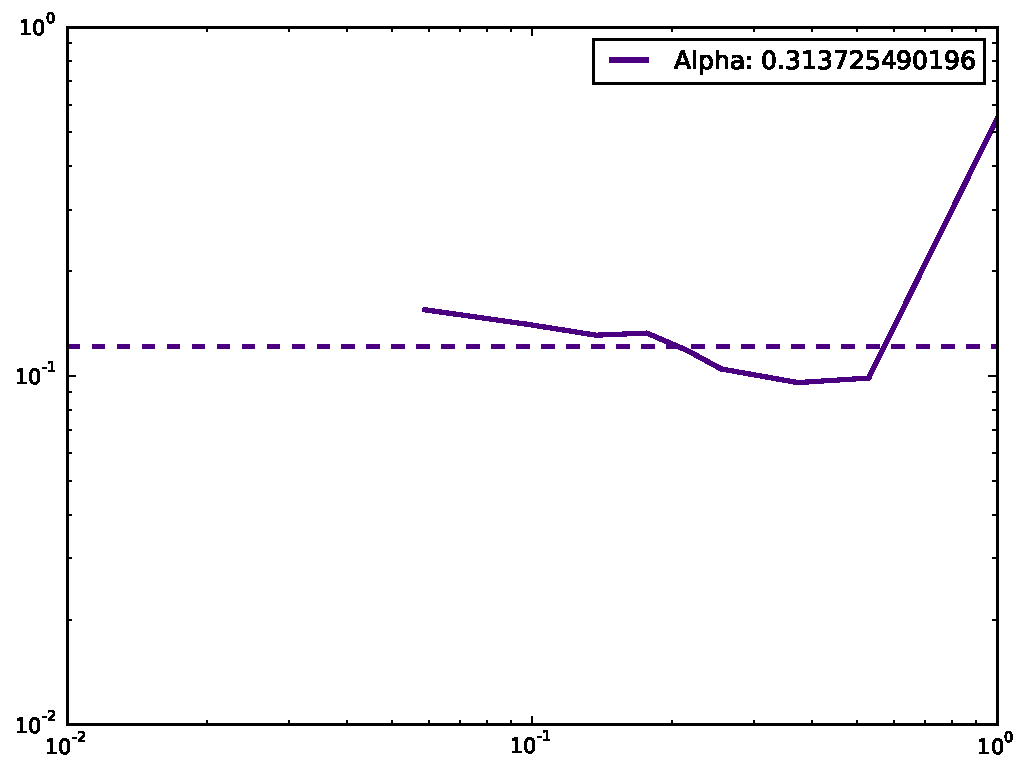
\includegraphics[scale=0.4]{images/algorithm/patch-0313.pdf}
\caption{Volatility plotted versus $\beta$ for $\alpha=0.313$}
\label{fig:beta alpha 0.3}
\end{figure}

\subsubsection{Case of critical $\alpha$ value}

Even though by looking at \ref{fig:beta alpha 0.3} it seems that community games win even when the critical value of $\alpha$ is considered, from our simulations different value of $\alpha_c$ has been estimated.
In our case $\alpha_c$ was estimated to be $0.6336$ and when community games are confronted with basic models a different picture arises that we can see in Figure \ref{fig:beta alpha critical}.
This time community games are worse off whatever the $\beta$ value is when compared to basic MGs.
One of the possible and plausible explanations for this phenomenon could be that when critical value for $\alpha$ is used information is exploited in an optimal way, and by implementing communities half of the bits of brain size are taken up by the community minority game that artificially lower the $\alpha$ moving it from its optimal value $\alpha_c$, hence making the system a bit more inefficient.
However this approach to studying the community aspect has not been elaborated in detail, so future studies are necessary before further explanations are proposed or present one confirmed.

\begin{figure}[h]
\centering
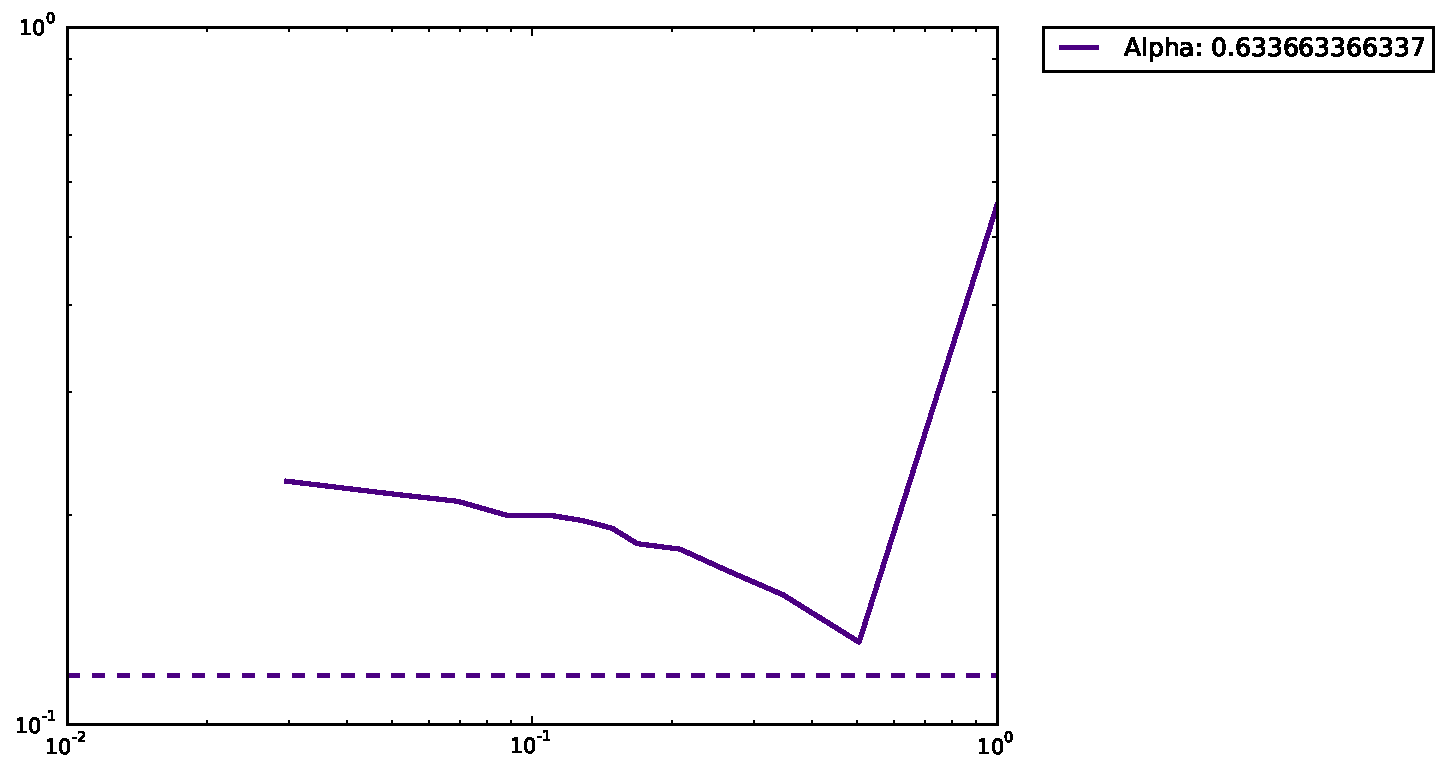
\includegraphics[scale=0.4]{images/algorithm/patch-063.pdf}
\caption{Volatility plotted versus $\beta$ for $\alpha_c$}
\label{fig:beta alpha critical}
\end{figure}

In certain cases we have still think community games should be used even when critical value of $\alpha$ is obtained.
A simple consideration of reliability of the information helps us explain why we support community based approach.
If no communities are used, only temporal information from the global game is available.
In a case where the network structure is rather dynamic with different agents joining and leaving the game, different optimal strategies may arise.
By constructing the model that considers the communities we could obtain more robustness to the ever changing nature of the system.
In case where the agents, their number and all their parameters are static, and $\alpha$ is at its critical value, most probably community implementation would worsen the volatility.

The affirmations presented in the last few paragraphs are based on intuition developed during this work, and have not been backed up by computational simulation.
We offer them more as a plausible explanation that should be confirmed by further experiments.

\subsection{Optimal number of communities}
\label{subsec:optimal beta}

For each value of $\alpha$ different optimal value of $\beta$ is found.
This means that for different conditions of the system, defined by the number of agents and their cognitive abilities, we can find an optimal number of communities that the system should be divided into.
The Figure \ref{fig:optimal beta} shows the optimal $\beta$ values for $\alpha$ in the range $[0.1,2.5]$.
We have drawn the $\alpha_c$ with a vertical dotted line that divides the basic minority game in two phases described in \ref{subsec:phasetransition}.
We can see that for $\alpha$ values smaller than $\alpha_c$ the optimal value of $\beta$ is between $0.1$ and $0.35$, which tells us that the set of agents should be divided in a number of communities ranging from $3$ to $10$ in order to optimize the model.
Around $\alpha_c$ and when $\alpha>\alpha_c$ our best estimate is to divide the set of agents in two communities.
These communities should be exclusive and should contain half the agents each, in order to evade the repetitive information that is included in both communities.
This is just a different way of  saying that the communities should be isolated.

\begin{figure}[h]
\centering
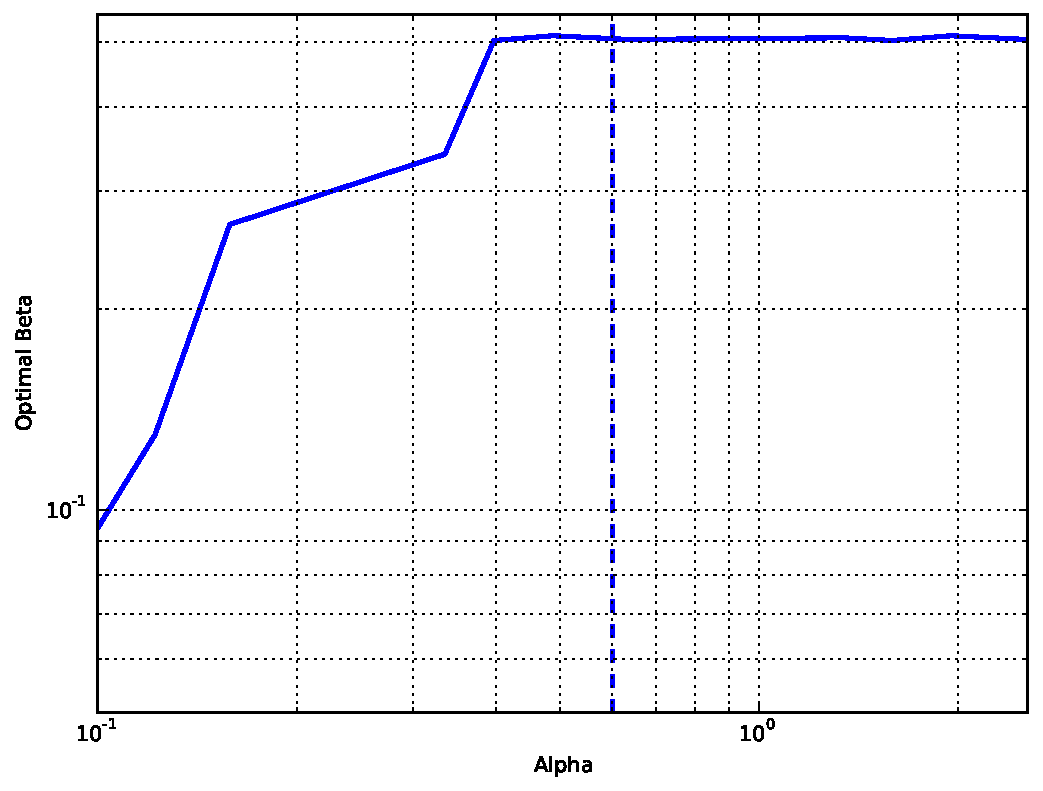
\includegraphics[scale=0.4]{images/algorithm/optimal_beta.pdf}
\caption{Optimal values of $\beta$ versus various values of $\alpha$}
\label{fig:optimal beta}
\end{figure}

To sum up, we are to prefer a community structure to basic minority model and we can estimate the number of communities to be used if some parameters of the model are known.

\subsection{Hierarchical topology}
\label{subsec:hierarchical}

When possible, fixed patch communities should be preferred as they perform much better than other network structures.
However not always it is possible to construct communities with all agents interconnected inside the community and not connected to any other agent outside its own community.
An example could be a computer network, where certain nodes are peripheral and not connected directly to most of other nodes.
This forces us to use a central control unit for each community, that defies the whole concept of decentralized system of resource allocation, or to use scale free network model instead of fixed patch.

We propose a new approach to construct the network of minority agents based on a hybrid approach using two techniques presented in Sections \ref{sec:scale free} and \ref{sec:small world}.
Small world and scale free graphs allow us to model more realistically human and computer networks, but they still have certain fallacies.
Scale free networks simulate the popularity effect through its peripheral attachment mechanism, making certain nodes more probable to have higher degree with respect to others.
However scale free network do not enable us to simulate high clustering around the whole network, clustering is generated only at the \textit{central} nodes, the ones with high degree.
On the other hand, small world graphs have high clustering property, intrinsic in it's algorithm definition, but the degree of each node is the same.
We call this new topology hierarchical.

The peripheral attachment, the defining property of scale free networks, seems present in most systems studied for the purpose of this thesis, for example a computer network with routers acting as hubs and end users as less-popular agents.
Likewise the clustering is also a real phenomenon, for example different branches of financial markets form loosely connected communities, divided whether by the object of their trading or by the place of their operation.
These phenomenons can make the division in fixed patch communities harder and a different approach is used, that exploits the nature of human and computer networks enhanced with the knowledge of optimal $\beta$ described in subsection \ref{subsec:optimal beta}.

The optimal value of $\beta$ is used to divide the set of agents in $C$ communities.
Single communities are formed by using the Barabasi-Albert algorithm in order to obtain the peripheral attachment property.
After $C$ communities have been generated they are united in a larger community and a second step of the Watts-Strogatz algorithm is executed to create a short average length between different communities.
If a high enough degree parameter is given to the Barabasi-Albert algorithm we can obtain locally high clustering, while maintaining the short average length between nodes with Watts-Strogatz application to the entire network.

\begin{figure}[h]
\centering
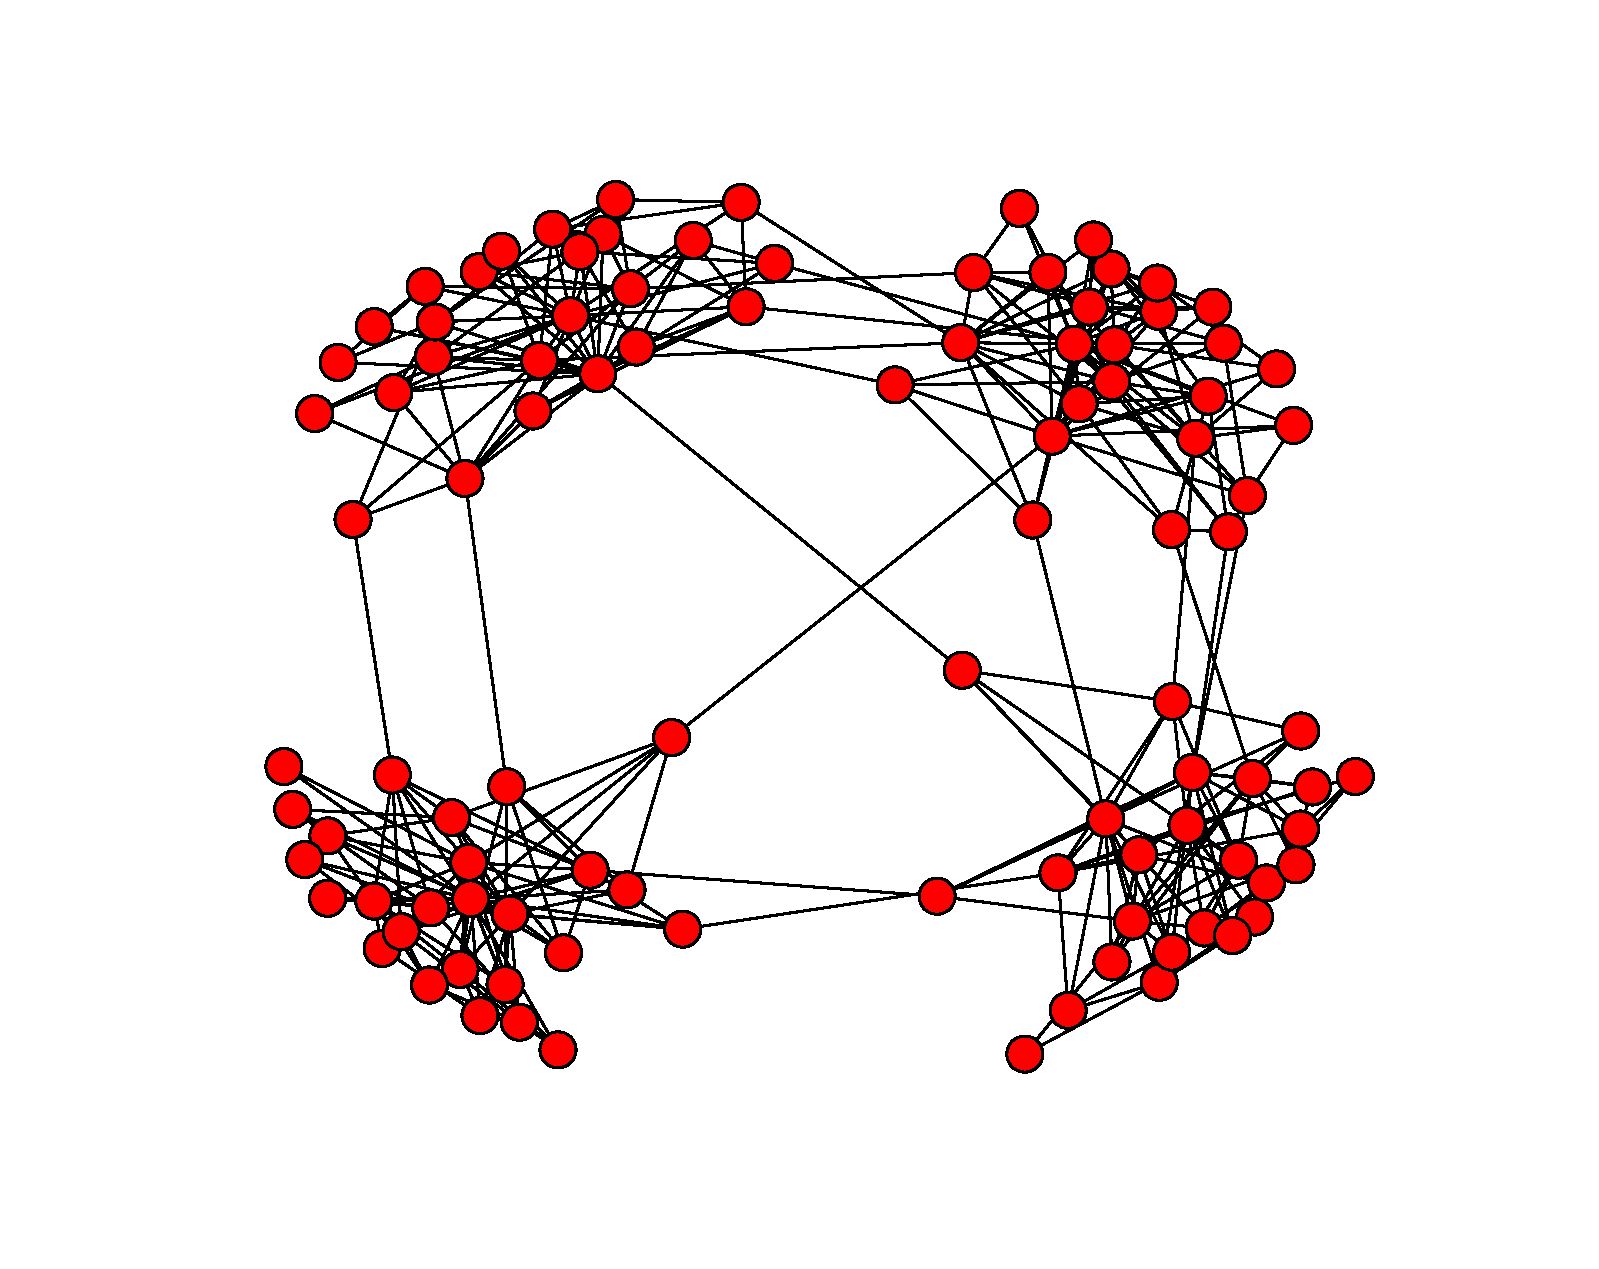
\includegraphics[scale=0.4]{images/topology/hierarchical_graph_4_dot05.pdf}
\caption{Hierarchical graph with $N=101$, $C=4$, $K=4$ and $\beta = 0.05$}
\label{fig:hierarchical graph 4}
\end{figure}

An example of a hierarchical graph can be seen in Figure \ref{fig:hierarchical graph 4} where $101$ initial agents are first divided into $4$ communities and then each edge is rewired with $\beta=0.05$ probability. 
The 4 communities are clearly visible and each community is loosely linked to each other maintaining low the short average path.

Same observation can be made by looking at the adjacency matrix of different hierarchical graphs.
Examples for hierarchical graphs with $C$ in $\{2,3,4\}$ for $\beta=0.1$ are visible in Figure  \ref{fig:hierarchical adjacency graph 0.1}, while for the same number of communities but with higher rewiring parameter $\beta=0.25$ can be seen in Figure \ref{fig:hierarchical adjacency graph 0.25}.

\begin{figure}[h]
        \centering
        \begin{subfigure}[b]{0.3\textwidth}
        	\centering
                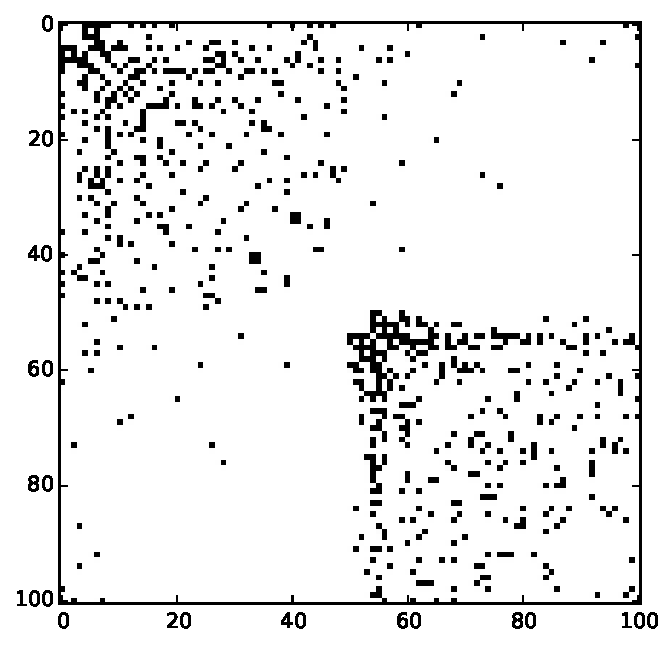
\includegraphics[width=\textwidth]{images/topology/hierarchical_adjacency_2_dot1.pdf}
                \caption{$C=2$}
        \end{subfigure}
        \begin{subfigure}[b]{0.3\textwidth}
        	\centering
                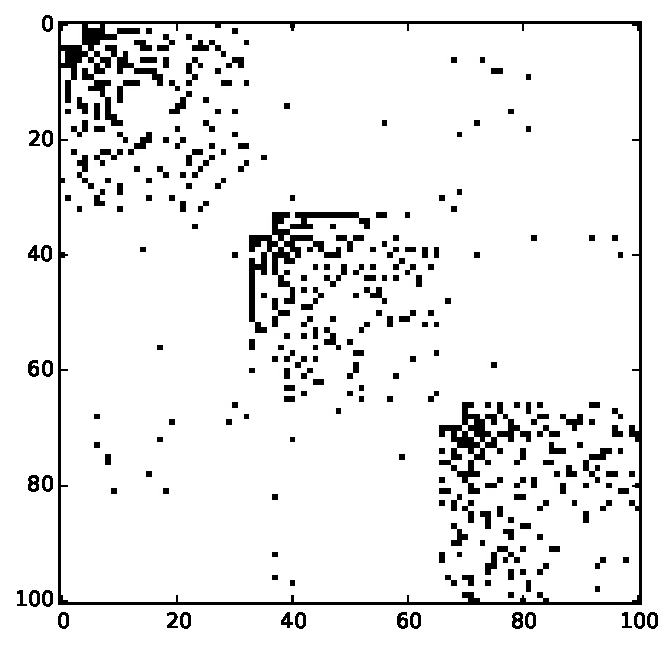
\includegraphics[width=\textwidth]{images/topology/hierarchical_adjacency_3_dot1.pdf}
                \caption{$C=3$}
        \end{subfigure}
        \begin{subfigure}[b]{0.3\textwidth}
        	\centering
                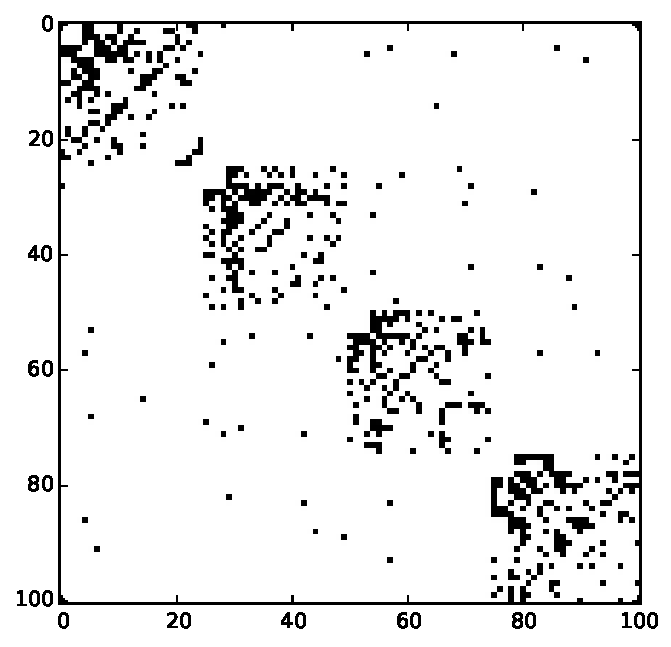
\includegraphics[width=\textwidth]{images/topology/hierarchical_adjacency_4_dot1.pdf}
                \caption{$C=4$}
        \end{subfigure}
        \caption{Hierarchical graph adjacency matrices with $N=101$, $K=5$ and $\beta =0.1$}
        \label{fig:hierarchical adjacency graph 0.1}
\end{figure}


\begin{figure}[h]
        \centering
        \begin{subfigure}[b]{0.3\textwidth}
        	\centering
                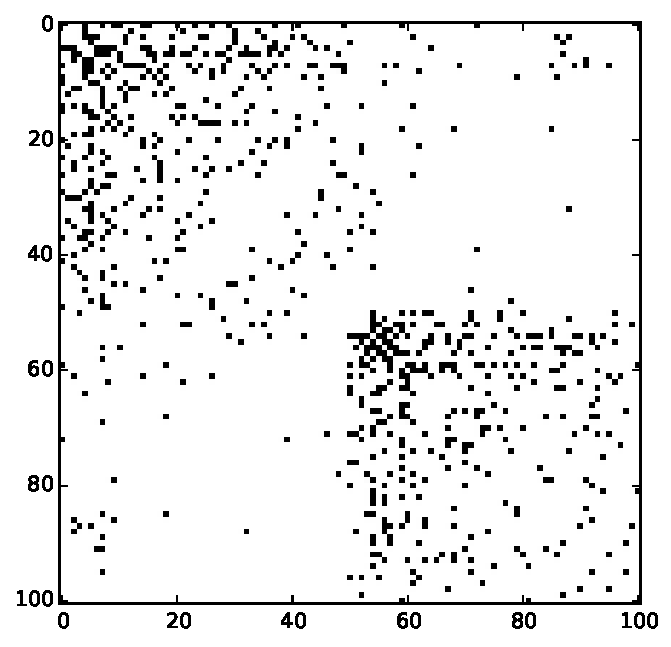
\includegraphics[width=\textwidth]{images/topology/hierarchical_adjacency_2_dot25.pdf}
                \caption{$C=2$}
        \end{subfigure}
        \begin{subfigure}[b]{0.3\textwidth}
        	\centering
                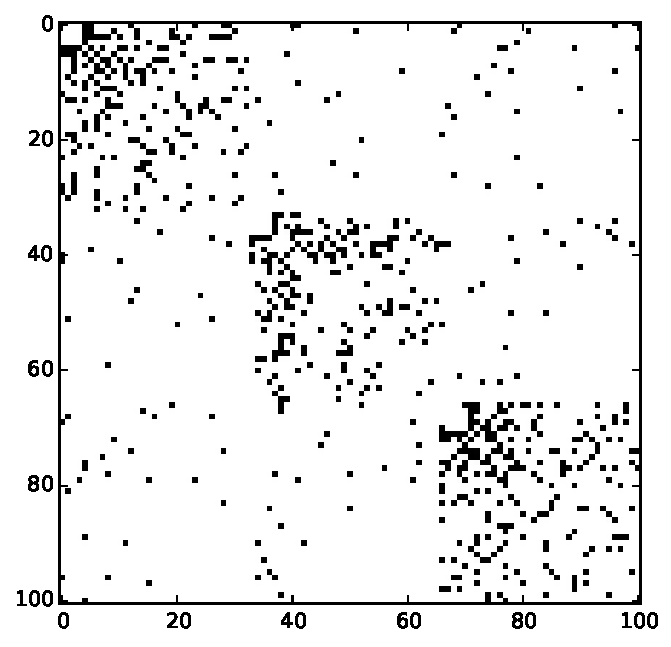
\includegraphics[width=\textwidth]{images/topology/hierarchical_adjacency_3_dot25.pdf}
                \caption{$C=3$}
        \end{subfigure}
        \begin{subfigure}[b]{0.3\textwidth}
        	\centering
                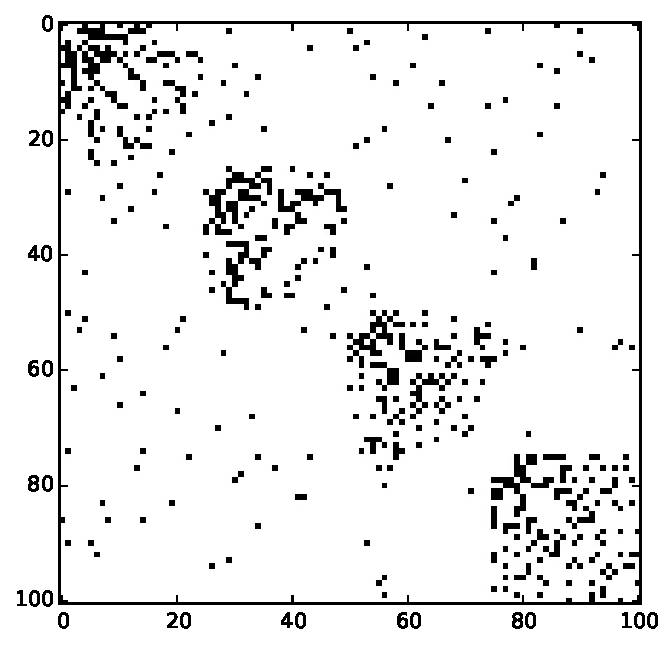
\includegraphics[width=\textwidth]{images/topology/hierarchical_adjacency_4_dot25.pdf}
                \caption{$C=4$}
        \end{subfigure}
        \caption{Hierarchical graph adjacency matrices with $N=101$, $K=5$ and $\beta =0.25$}
        \label{fig:hierarchical adjacency graph 0.25}
\end{figure}

\subsection{The algorithm}
\label{subsec:algorithm}

Equipped with the knowledge of the optimal number of communities a set of agents should be divided into and other assumption made, primarily that using community based agents make the model more robust, we can define an algorithm to create a network structure of a hierarchical type described in detail in \ref{subsec:hierarchical}.
This algorithm is to be used when full fixed patch topology is not practical.

\quad
\begin{algorithm}[H]
\KwData{Number of Agents N, Brain size M}
\KwResult{Hierarchical network structure G, CG}
$\alpha \leftarrow \frac{2^M}{N}$\;
$\beta \leftarrow $optimalBeta($\beta$)\;
\For{$i \in [1,\frac{N}{N\beta}]$}{
	$C_i \leftarrow $generateBarabasiAlbertGraph$(N * \beta, 0.5 * N * \beta)$\;
	\For{$j \in E(C_i)$}{
		Rewire $j$ with $P=0.1$\;
	}
	$CG_i \leftarrow $generateCommunityGame($C_i$)\; 
}
$G \leftarrow $generateGlobalGame()\;
return G, CG\;
\quad
\caption{Hierarchical MG algorithm}
\end{algorithm}
\quad

Note that we have decided to use $0.5 * N * \beta$, ie. half of the number of agents in a community, as a parameter $K$ for Barabasi-Albert algorithm because in that way we can obtain highly clustered communities with high average degree of nodes.
This parameter should be evaluated when real world structure poses certain limits to this kind of topology, and if no such restrictions are present this estimate is a good one.
Another fixed parameter inserted in the algorithm is the rewiring probability set to $0.1$, from initial estimates, but further analysis could prove other values to be more desirable.

\section{Real world applications}
\label{sec:real world}

We have mentioned possible applications of the MG model in real world problems and how our results could help better the already proposed solutions.
In this Section we briefly present various models proposed by different authors to exploit the decentralized and cooperative properties of minority games to make a more efficient resource allocation systems.

\subsection{Financial markets}
\label{subsec:financial markets}

A brief excursus has been made into modelling the financial markets in Chapter \ref{chapter:minority}, and more specifically in Section \ref{minority:variations}, so we will not engage in a repetitive description of how markets are modelled.

Although minority games have been primarily used to model financial markets, our results are more easily implemented in other cases.
The reason for this is that we have assumed to be the architects of network structures studied, where we can decide how to partition the set of agents in different communities.
This sort of action is rather difficult in today's financial markets, and is a responsibility of other institution to reorganize the stock exchange in order to lower the volatility.

However, the results from this thesis could prove to be an interesting investment strategy if one is inclined to try it, acting as a single agent inside the market.
By applying the same procedure presented in Section \ref{sec:proposed algorithm}, a trading strategy could constructs a fixed community, which dimension would be defined by the dimension of the market and the medium assumed rounds taken into account by other agents.
This community could serve as a \textit{reliability factor} that the trading strategy uses to predict future outcomes of the market.

\subsection{Delay Tolerant Networks}
\label{subsec:dtn}

Different works have recently proposed to use a minority games inspired model for Delay Tolerant Networks (DTNs), mainly \cite{sidi2012incentive} and \cite{sidi2013coordination}.
These sort of networks are characterized by the trying to resolve technical issues that emerge from heterogeneous networks that lack in continuous communication.
Perfect examples are networks operating in mobile or extreme terrestrial environments.
Main properties are the absence of dedicated infrastructure and a message replication mechanism.
Absence of infrastructure is resolved by using nodes inside the network as a support for all the communication, this is made easy in case of mobile networks as new systems already include the APIs for information exchange between nodes.
This information exchange can be used as information carrier to offload infrastructure in case of overloading.
Message replication mechanism, also called epidemic routing protocol, means that messages are replicated in many instances from source to destination.
As no feedback mechanism is defined, the best way to increase the probability of the destination node to receive the original message is to have it replicated as many times as possible.

This raises the problem that can be modelled with minority games.
When a node source (S) sends a message to a node destination (D), the message gets replicated as many times as possible, but only the first message that arrives to D is useful, as all the other replicas are discarded once they arrive at D.
This can prove to be a waste of resources, be it energy used to forward the messages, or the time consumed that could have been used better.
Since the central system is not present per definition, an agent based approach seems like the most plausible one.

Minority games can be implemented to render this system more efficient.
Every node has to decide when a message is received if it should use its resources to transmit this message of simply drop it.
In the case of DTNs only the nodes that have participated in making the first message arrive to node D are awarded points, while all the rest of the nodes that have forwarded the message but are not in the final path route are defined losers.
Awarded points in these networks could be some form of currency that enables the nodes to transmit their own messages and become node S.
So how should a node decide whether to participate or not in the message chain? 
Simplest mechanism is to keep track of history of personal decisions and implement basic $S$ strategies as defined in Chapter \ref{chapter:minority}.

We think a further step could be added, where simple communities are formed by nearby nodes.
With the standard information exchange between nodes additional minority information could be exchanged to lower the waste of resources inside this model.

%\subsection{Smart energy resource allocation}
%\label{subsec:smart energy}

%Energy management systems (EMS) are automatic controllers for buildings that have more than one energy resource available.
%Zhang et al. have proposed a minority based model for energy allocation in smart buildings to make a more efficient use of renewable solar energy and lower the consumption of main grid electricity in \cite{zhang2012fair}.

%Currently energy management systems are centralized and static in their decision making.
%This means that energy peak consumption and energy peak generation are barely optimized, and since a static distribution of energy resource is implemented, changes in renewable energy generation are not predicted and optimized.

%Main components of a EMS system for smart buildings are: solar PV panels, access to main grid, energy storage system and power converters.
%Zhang et al. propose an model of a minority game where the whole game is represented by the entire building and single apartments are agents in the game.
%To make it possible, for each apartment an addition of a smart power meter is required, that makes the estimation of the local profile of the apartment energy consumption, and acts as an agent.

%The mechanism is simple and as follows, at every interval of time $t$ an estimate of the personal energy consumption is made by using previous data collected inside the apartment.


\subsection{Computer resource allocation}
\label{subsec:computer resource}

In computer systems different processes compete for different resources.
How these resources are distributed decides how fast the computer operates and raises its value.
So in our attempt to simulate a competitive system with agent based approach and limited resources, we can think of a single process as an agent and the computer resource capacity as the minority rule.
This means that when more that the resource capacity is asked for the system is overloaded, while if the quantity of resources required at certain moment is rather low a system can be considered idle.
The optimal situation would be to have a resource used as closely as possible to its limit.

Lam et al. have worked on a model based on minority games that simulates the optimal allocation of computer resources to the processes in \cite{lam2007adaptive}.
They propose a simple minority game model where at each round agents decide whether to ask for resource $R$ with limited capacity $C$ based on their strategies.
After all the agents have made their decision if resource $R$ is not overloaded, the agents that have chosen to use $R$ are awarded points, while when $R$ is overloaded the agents that have chosen not to use it are awarded points.
They further extend their model to a multi-resource/multi-choice model.

During this thesis we have worked on single-choice models, and our results could be tested with a single-choice model of computer resource allocation.
Interesting experiment could be to test if certain community structures arise in multi-choice models, that maybe result in models being more efficient when agents that prevalently use the same resources are put in the same communities.